\chapter{Fibered categories and Stacks}
\begin{center}
	{\huge Speaker: Francesco Sorce}
\end{center}
\bigskip

\noindent
Everything in this chapter is talked about in greater detail in \cite{vistoli2007notesgrothendiecktopologiesfibered}.

\section{Fibered categories}
\subsection{Definition}
\begin{definition}[]
If we have the data of $\Fc$ and $\Cc$ two categories and $p_\Fc:\Fc\to \Cc$ a functor we say that $\Fc$ is \textbf{over} $\Cc$.

In this context, if $p_\Fc(\xi)=U$ for some object $\xi$ we say that $\xi$ is over $U$. 

Similarly if $p_\Fc(\xi\to \eta)=U\to V$ then $\xi\to \eta$ is over $U\to V$.
\end{definition}

\begin{notation}
In the diagrams that follow, a normal or dashed arrow will be a morphism, while an allow with a tail (like $\mapsto$) represents applying the functor.
\end{notation}


\begin{definition}[]
An arrow $\phi:\xi\to \eta$ in $\Fc$ over $\Cc$ is \textbf{cartesian} if for all $\phi:\zeta\to \eta$ and all $h:p_\Fc\zeta\to p_\Fc\xi$ which make the following diagram commute there exists a unique arrow $\zeta\to \xi$ in place of the dotted arrow:
% https://q.uiver.app/#q=WzAsNixbMSwxLCJcXHhpIl0sWzIsMSwiXFxldGEiXSxbMSwyLCJVIl0sWzIsMiwiViJdLFswLDAsIlxcemV0YSJdLFswLDEsIlciXSxbMCwxLCJcXHBoaSJdLFsyLDNdLFswLDIsIiIsMSx7InN0eWxlIjp7InRhaWwiOnsibmFtZSI6Im1hcHMgdG8ifX19XSxbMSwzLCIiLDEseyJzdHlsZSI6eyJ0YWlsIjp7Im5hbWUiOiJtYXBzIHRvIn19fV0sWzQsMSwiXFxwc2kiLDAseyJjdXJ2ZSI6LTF9XSxbNSwyLCJoIl0sWzQsNSwiIiwwLHsic3R5bGUiOnsidGFpbCI6eyJuYW1lIjoibWFwcyB0byJ9fX1dLFs0LDAsIiIsMSx7InN0eWxlIjp7ImJvZHkiOnsibmFtZSI6ImRhc2hlZCJ9fX1dLFs1LDMsIiIsMSx7ImN1cnZlIjotMX1dXQ==
\[\begin{tikzcd}
	\zeta \\
	W & \xi & \eta \\
	& U & V
	\arrow[maps to, from=1-1, to=2-1]
	\arrow[dashed, from=1-1, to=2-2]
	\arrow["\psi", curve={height=-6pt}, from=1-1, to=2-3]
	\arrow["h", from=2-1, to=3-2]
	\arrow[curve={height=-6pt}, from=2-1, to=3-3]
	\arrow["\phi", from=2-2, to=2-3]
	\arrow[maps to, from=2-2, to=3-2]
	\arrow[maps to, from=2-3, to=3-3]
	\arrow[from=3-2, to=3-3]
\end{tikzcd}\]
If $\xi\to \eta$ is cartesian and over $f:U\to V$ we say that $\xi$ is the \textbf{pullback of $\eta$ along $f$}. We may write $\xi=f^\ast \eta$ if we fix a choice of pullback.
\end{definition}

\begin{definition}
Let us fix a category $\Cc$. The associated \textbf{arrow category} $\Arr(\Cc)$ is the category whose objects are arrows in $\Cc$ and whose morphisms are commutative squares in $\Cc$.
\end{definition}
\begin{remark}
We may view $\Arr(\Cc)$ as a category over $\Cc$ by fixing the functor that to an arrow $X\to U$ assigns $U$.
\end{remark}

\begin{example}
In order to better understand cartesian arrows (and to see where the name comes from) we determine which arrows in $\Arr(\Cc)$ are cartesian.

If an arrow $(X\to U)\to (Y\to V)$ is cartesian, consider the following data:
% https://q.uiver.app/#q=WzAsNSxbMiwxLCJZIl0sWzEsMiwiVSJdLFsyLDIsIlYiXSxbMSwxLCJYIl0sWzAsMCwiWiJdLFsxLDJdLFswLDIsIiIsMSx7InN0eWxlIjp7InRhaWwiOnsibmFtZSI6Im1hcHMgdG8ifX19XSxbMywwXSxbMywxXSxbNCwwXSxbNCwxXV0=
\[\begin{tikzcd}
	Z \\
	& X & Y \\
	& U & V
	\arrow[from=1-1, to=2-3]
	\arrow[from=1-1, to=3-2]
	\arrow[from=2-2, to=2-3]
	\arrow[from=2-2, to=3-2]
	\arrow[maps to, from=2-3, to=3-3]
	\arrow[from=3-2, to=3-3]
\end{tikzcd}\]
which we may equivalently rewrite
% https://q.uiver.app/#q=WzAsOSxbMiwxLCJZIl0sWzEsMiwiVSJdLFsyLDIsIlYiXSxbMSwxLCJYIl0sWzAsMCwiWiJdLFswLDEsIloiXSxbMiwzLCJWIixbMCwwLDQ5LDFdXSxbMSwzLCJVIixbMCwwLDQ5LDFdXSxbMCwyLCJaIixbMCwwLDQ5LDFdXSxbMSwyXSxbMCwyLCIiLDEseyJzdHlsZSI6eyJ0YWlsIjp7Im5hbWUiOiJtYXBzIHRvIn19fV0sWzMsMF0sWzMsMV0sWzQsMF0sWzQsNSwiaWRfWiIsMl0sWzUsMl0sWzIsNiwiIiwxLHsiY29sb3VyIjpbMCwwLDQ5XSwic3R5bGUiOnsidGFpbCI6eyJuYW1lIjoibWFwcyB0byJ9fX1dLFs3LDYsIiIsMSx7ImNvbG91ciI6WzAsMCw0OV19XSxbMSw3LCIiLDEseyJjb2xvdXIiOlswLDAsNDldLCJzdHlsZSI6eyJ0YWlsIjp7Im5hbWUiOiJtYXBzIHRvIn19fV0sWzgsNywiIiwxLHsiY29sb3VyIjpbMCwwLDQ5XX1dLFs4LDYsIiIsMSx7ImNvbG91ciI6WzAsMCw0OV19XSxbNSw4LCIiLDEseyJjb2xvdXIiOlswLDAsNDldLCJzdHlsZSI6eyJ0YWlsIjp7Im5hbWUiOiJtYXBzIHRvIn19fV1d
\[\begin{tikzcd}
	Z \\
	Z & X & Y \\
	\textcolor{rgb,255:red,125;green,125;blue,125}{Z} & U & V \\
	& \textcolor{rgb,255:red,125;green,125;blue,125}{U} & \textcolor{rgb,255:red,125;green,125;blue,125}{V}
	\arrow["{id_Z}"', from=1-1, to=2-1]
	\arrow[from=1-1, to=2-3]
	\arrow[color={rgb,255:red,125;green,125;blue,125}, maps to, from=2-1, to=3-1]
	\arrow[from=2-1, to=3-3]
	\arrow[from=2-2, to=2-3]
	\arrow[from=2-2, to=3-2]
	\arrow[maps to, from=2-3, to=3-3]
	\arrow[color={rgb,255:red,125;green,125;blue,125}, from=3-1, to=4-2]
	\arrow[color={rgb,255:red,125;green,125;blue,125}, from=3-1, to=4-3]
	\arrow[from=3-2, to=3-3]
	\arrow[color={rgb,255:red,125;green,125;blue,125}, maps to, from=3-2, to=4-2]
	\arrow[color={rgb,255:red,125;green,125;blue,125}, maps to, from=3-3, to=4-3]
	\arrow[color={rgb,255:red,125;green,125;blue,125}, from=4-2, to=4-3]
\end{tikzcd}\]
Since the arrow is cartesian, there is a unique way to complete the diagram above with maps $Z\to X$ and $Z\to U$. Since we ask for compatibility with the functor, $Z\to U$ is already known, so we have constructed $Z\to X$ in the first diagram. This makes us suspect that cartesian arrows in $\Arr(\Cc)$ correspond to cartesian squares in $\Cc$, and this is true.

Indeed, suppose that $(X\to U)\to (Y\to V)$ is a cartesian square and let us consider the data
% https://q.uiver.app/#q=WzAsOSxbMiwxLCJZIl0sWzEsMiwiVSJdLFsyLDIsIlYiXSxbMSwxLCJYIl0sWzAsMCwiWiJdLFswLDEsIlciXSxbMiwzLCJWIixbMCwwLDQ5LDFdXSxbMSwzLCJVIixbMCwwLDQ5LDFdXSxbMCwyLCJXIixbMCwwLDQ5LDFdXSxbMSwyXSxbMCwyLCIiLDEseyJzdHlsZSI6eyJ0YWlsIjp7Im5hbWUiOiJtYXBzIHRvIn19fV0sWzMsMF0sWzMsMV0sWzQsMF0sWzQsNV0sWzUsMl0sWzIsNiwiIiwxLHsiY29sb3VyIjpbMCwwLDQ5XSwic3R5bGUiOnsidGFpbCI6eyJuYW1lIjoibWFwcyB0byJ9fX1dLFs3LDYsIiIsMSx7ImNvbG91ciI6WzAsMCw0OV19XSxbMSw3LCIiLDEseyJjb2xvdXIiOlswLDAsNDldLCJzdHlsZSI6eyJ0YWlsIjp7Im5hbWUiOiJtYXBzIHRvIn19fV0sWzgsNywiIiwxLHsiY29sb3VyIjpbMCwwLDQ5XX1dLFs4LDYsIiIsMSx7ImNvbG91ciI6WzAsMCw0OV19XSxbNSw4LCIiLDEseyJjb2xvdXIiOlswLDAsNDldLCJzdHlsZSI6eyJ0YWlsIjp7Im5hbWUiOiJtYXBzIHRvIn19fV1d
\[\begin{tikzcd}
	Z \\
	W & X & Y \\
	\textcolor{rgb,255:red,125;green,125;blue,125}{W} & U & V \\
	& \textcolor{rgb,255:red,125;green,125;blue,125}{U} & \textcolor{rgb,255:red,125;green,125;blue,125}{V}
	\arrow[from=1-1, to=2-1]
	\arrow[from=1-1, to=2-3]
	\arrow[color={rgb,255:red,125;green,125;blue,125}, maps to, from=2-1, to=3-1]
	\arrow[from=2-1, to=3-3]
	\arrow[from=2-2, to=2-3]
	\arrow[from=2-2, to=3-2]
	\arrow[maps to, from=2-3, to=3-3]
	\arrow[color={rgb,255:red,125;green,125;blue,125}, from=3-1, to=4-2]
	\arrow[color={rgb,255:red,125;green,125;blue,125}, from=3-1, to=4-3]
	\arrow[from=3-2, to=3-3]
	\arrow[color={rgb,255:red,125;green,125;blue,125}, maps to, from=3-2, to=4-2]
	\arrow[color={rgb,255:red,125;green,125;blue,125}, maps to, from=3-3, to=4-3]
	\arrow[color={rgb,255:red,125;green,125;blue,125}, from=4-2, to=4-3]
\end{tikzcd}\]
then we have a unique way to complete the diagram. The bottom map is determined by compatibility with the functor towards $\Cc$ and the top arrow can be chosen to be the one induced by the fact that we have a cartesian square an maps $Z\to Y$, $Z\to U$, where the second one is the composition $Z\to W\to U$.
\end{example}


\begin{fact}\label{FctCartArrow}
Cartesian arrows satisfy the following properties:
\begin{enumerate}
\item the composition of cartesian arrows is cartesian
\item if $\xi\to \zeta$ factors through $\eta$ with $\eta\to \zeta$ being cartesian, then $\xi\to \zeta$ is cartesian if and only if $\xi\to \eta$ is
\item if $\phi$ is over an isomorphism then $\phi$ is cartesian if and only if it is an isomorphism
\end{enumerate}
\end{fact}

\begin{definition}[]
A category $\Fc$ over $\Cc$ is \textbf{fibered over $\Cc$} if for all $f:U\to V$ in $\Cc$ and all $\eta\in \Fc$ over $V$ there exists a cartesian arrow $\phi:\xi\to \eta$ over $f$. That is, given a ``partial diagram" of the form
% https://q.uiver.app/#q=WzAsMyxbMSwwLCJcXGV0YSJdLFswLDEsIlUiXSxbMSwxLCJWIl0sWzEsMiwiZiJdLFswLDIsIiIsMSx7InN0eWxlIjp7InRhaWwiOnsibmFtZSI6Im1hcHMgdG8ifX19XV0=
\[\begin{tikzcd}
	& \eta \\
	U & V
	\arrow[maps to, from=1-2, to=2-2]
	\arrow["f", from=2-1, to=2-2]
\end{tikzcd}\]
we can make it a square in such a way that the top side is a cartesian arrow.
\end{definition}

\begin{definition}[]
Let $\Fc$ and $\Gc$ be fibered categories over $\Cc$. A \textbf{morphism of fibered categories over $\Cc$} from $\Fc$ to $\Gc$ is a functor $F:\Fc\to \Gc$ such that $p_\Gc\circ F=p_\Fc$ which preserves cartesian arrows, i.e. if $\phi\in \Fc$ cartesian then $F(\phi)$ is cartesian in $\Gc$.
\end{definition}

\begin{example}
Because of what we have already said, $\Arr(\Cc)$ is fibered over $\Cc$ if and only if $\Cc$ admits fibered products.
\end{example}

\subsection{Fibers}
We now reach one of the main definitions which motivate fibered categories

\begin{definition}[]
Let $\Fc$ be a fibered over $\Cc$ and fix an object $U\in \Cc$. The \textbf{fiber of $\Fc$ over $U$} is the subcategory $\Fc(U)$ of $\Fc$ whose objects are the objects of $\Fc$ over $U$ and whose morphisms are those \ul{over $id_U$}.
\end{definition}

\begin{example}
Fix $U\in \Cc$. The fiber $\Arr(\Cc)(U)$ is the comma category $\Cc/U$.
\end{example}

\begin{remark}
If $f:U\to V$ is a morphism in $\Cc$ and $\Fc$ is fibered over $\Cc$ then we may define a ``restriction functor"
\[\funcDef{\Fc(V)}{\Fc(U)}{X}{f^\ast X}\]
upon choosing a unique pullback for each element. Such a choice is called a \textbf{cleavage}. For more details see \cite{vistoli2007notesgrothendiecktopologiesfibered}.
\end{remark}

\begin{remark}
If $F:\Fc\to \Gc$ is a morphism of fibered categories over $\Cc$ and $U\in \Cc$ then it induces a functor $F_U:\Fc(U)\to \Gc(U)$.
\end{remark}

\begin{center}
    \textit{These definitions make $\Fc$ look like a presheaf $\Cc\op\to \Cat$}
\end{center}

\noindent This is not quite correct because choosing a cleavage may lead to having two arrows that should be the same being naturally isomorphic instead. To be technically correct we would need to introduce pseudo-functors, but they behave like normal functors in basically every way.


\begin{fact}
There is a correspondence between categories fibered over $\Cc$ and pseudo-functors $\Cc\op\to \Cat$.
\end{fact}
\begin{proof}[Proof (Idea)]
To get the functor from the category fix a cleavage, then take an object to the fiber over it and a map to the pullback along it.
\medskip

\noindent
To get a category from the functor consider the category with objects $(U,X)$ for $U\in \Cc$ and $X\in \Fc(U)$ and morphisms defined in the obvious way. The functor from this category to $\Cc$ is the projection on the first factor. The fact that this comes from a pseudo-functor automatically gives the existence of pullbacks.
\end{proof}

\begin{definition}[]
A category is called a \textbf{set} if its objects form a set and the only morphisms are of the form $id_X$ for some object $X$ in the category.
\end{definition}

\begin{definition}[]
A category is called a groupoid if every arrow in the category is an isomorphism.
\end{definition}

\begin{definition}[]
Let $\Fc$ be a category fibered over $\Cc$. We say that $\Fc$ is
\begin{itemize}
    \item \textbf{fibered in sets} if $\Fc(U)$ is a set for all $U\in \Cc$
    \item \textbf{fibered in groupoids} if $\Fc(U)$ is a groupoid for all $U\in \Cc$.
\end{itemize}
\end{definition}

\begin{fact}
A cateogry is fibered in sets if and only if the associated pseudo-functor is a functor in the usual sense.
\end{fact}

\begin{example}
Let $\Cc$ be a (locally small) category and let us fix $X\in \Cc$. We have a functor $\Cc\to \Fun(\Cc\op,\Set)$ which maps $X$ to $h_X=\Hom_\Cc(\cdot, X)$. This functor defines a category fibered over $\Cc$. The objects of this category are pairs $(Y,Y\to X)$ (which we will identify with $Y\to X$ itself) and a morphism from $Y\to X$ to $Z\to X$ is an arrow $Y\to Z$ in $\Cc$ such that $Y\to X=Y\to Z\to X$.

The fiber of this category over $Y\in \Cc$ is $\cpa{Y\to X}=\Hom_\Cc(Y,X)$ but seen as a category. Since arrows in a fiber must be over the identify of the object of which they are the fiber, the only arrows in $\Hom(Y,X)$ are the identity of $Y$. This shows that the category we got from $X$ is fibered in sets, which is what we expected because it came from a functor.

Schematically, we have the following embeddings and equivalences
% https://q.uiver.app/#q=WzAsNSxbMCwwLCJcXENjIl0sWzEsMCwiXFxGdW4oXFxDY1xcb3AsXFxTZXQpIl0sWzIsMCwiXFx0ZXh0e0ZpYmVyZWR9L1xcQ2MiXSxbMSwxLCJcXHRleHR7UmVwcmVzZW50YWJsZX0iXSxbMiwxLCJcXHRleHR7RmliZXJlZCBpbiBzZXRzfSJdLFswLDEsIiIsMix7InN0eWxlIjp7InRhaWwiOnsibmFtZSI6Imhvb2siLCJzaWRlIjoidG9wIn19fV0sWzEsMiwiIiwyLHsic3R5bGUiOnsidGFpbCI6eyJuYW1lIjoiaG9vayIsInNpZGUiOiJ0b3AifX19XSxbMCwzLCJcXHNpbSIsMl0sWzEsNCwiXFxzaW0iLDJdLFszLDEsIiIsMix7InN0eWxlIjp7InRhaWwiOnsibmFtZSI6Imhvb2siLCJzaWRlIjoidG9wIn19fV0sWzQsMiwiIiwxLHsic3R5bGUiOnsidGFpbCI6eyJuYW1lIjoiaG9vayIsInNpZGUiOiJ0b3AifX19XV0=
\[\begin{tikzcd}
	\Cc & {\Fun(\Cc\op,\Set)} & {\text{Fibered}/\Cc} \\
	& {\text{Representable}} & {\text{Fibered in sets}}
	\arrow[hook, from=1-1, to=1-2]
	\arrow["\sim"', from=1-1, to=2-2]
	\arrow[hook, from=1-2, to=1-3]
	\arrow["\sim"', from=1-2, to=2-3]
	\arrow[hook, from=2-2, to=1-2]
	\arrow[hook, from=2-3, to=1-3]
\end{tikzcd}\]
\end{example}

\begin{proposition}
Let $\Fc$ be a category over $\Cc$ (we do not assume fibered). $\Fc$ is fibered in groupoids over $\Cc$ if and only if the following conditions hold:
\begin{enumerate}
\item every arrow in $\Fc$ is cartesian
\item given a partial diagram $f:U\to V$ and $\eta\in \Fc$ over $V$, the exists some $\phi:\xi\to\eta$ over $f$.
\end{enumerate}
\end{proposition}
\begin{proof}[Sketch]
If $\Fc$ is fibered in groupoids, 2. holds by fiberedness and 1. is a consequence of point 2 in fact \ref{FctCartArrow}.

Viceversa, if 1. and 2. hold then $\Fc$ is fibered. Since all arrows in a fiber are over an isomorphism (the identity of the object we are taking the fiber), again by fact \ref{FctCartArrow} we see that all arrows must be isomorphisms because they are cartesian.
\end{proof}




\section{Stacks}

Now that we have explored the formalism of fibered categories, let us see how it interacts with the notion of Grothendieck topology we dealt with in the previous chapter.

\subsection{Motivating example}
Let us consider the arrow category associated to the category of topological spaces $\Arr(\Top)$.
We may interpret objects in this category to be \textit{spaces lying above a base space}. In what follows it may be useful to imagine objects in this category to be things like covering maps or fiber bundles, though of course the notion of ``continuous maps" is much more general.

Taking this as our point of view, two concepts we may want to explore are the following:
\begin{itemize}
\item Suppose we have two objects over the same base space and an open cover for that base. Under what conditions can we construct a map between them locally?
\item Suppose we have an open cover and that for each element of the cover we have a space over it. Under what conditions can we glue these pieces to get an object over the entire base space?
\end{itemize}

\noindent Studying these questions will eventually lead us to what a prestack and a stack should be.

\bigskip

\noindent Recall that we have a standard Grothendieck topology on $\Top$ for which 
\[\Cov(U)=\cpa{\cpa{U_i\to U}\mid \text{jointly surjective open immersions}}.\]

\begin{notation}
We will write $U_{ij}$ instead of $U_i\cap U_j$ and similarly $U_{ijk}$ for triple intersections.
\end{notation}

\subsubsection{Gluing maps}
Suppose we fix $U\in \Top$ and an open cover\footnote{in the standard sense. Everything works the same with jointly surjective open immersions but the notation gets bothersome rather quickly.} $\cpa{U_i\to U}$. We also fix two objects $\xi:X\to U$ and $\eta:Y\to U$. The answer to our first question can be summerized in the following proposition:

\begin{proposition}
Let $U$, $\cpa{U_i}$, $\xi,\eta$ be as above. Suppose we have maps $f_i:\xi\ii(U_i)\to \eta\ii(U_i)$ for all $i$ such that 
\[f_i\res{\xi\ii(U_{ij})}=f_j\res{\eta\ii(U_{ij})},\] 
then there exists a unique $f:X\to Y$ which is compatible with the maps to $U$ and such that $f\res{\xi\ii(U_i)}=f_i$ for all $i$.
\end{proposition}

Notice that we may restate the proposition as

\begin{proposition}
The functor
\[\ul{\Hom}_U(X,Y):\funcDef{(\Top/U)\op}{\Set}{Z\to U}{\Hom_Z(X\times_U Z, Y\times_U Z)}\]
is a sheaf with respect to the Grothendieck topology induced by $\Top$ on $\Top/U$.
\end{proposition}

To see the equivalence, note that $X\times_U U_i=\xi\ii(U_i)$ and $Y\times_U U_i=\eta\ii(U_i)$, so when you evaluate the functor on the open cover of $U$, the fact that it is a sheaf corresponds exactly to the gluing property.

\subsubsection{Gluing spaces}

We now look at what it means to glue spaces using a cover:

\begin{proposition}
Let us fix a topological space $U$ together with an open cover $\cpa{U_i}$. For each $i$ let $u_i:X_i\to U_i$ be an element of $\Arr(\Top)$. We also fix isomorphisms $\phi_{ij}:u_j\ii(U_{ij})\to u_i\ii(U_{ij})$ for each pair of indices in such a way so that 
\[\phi_{ik}\res{u_k\ii(U_{ijk})}=\phi_{ij}\res{u_j\ii(U_{ijk})}\circ \phi_{jk}\res{u_i\ii(U_{ijk})}.\]
It follows that there exists $u:X\to U$ continuous, together with homeomorphisms $\phi_i:u\ii(U_i)\to X_i$ such that $\phi_{ij}=\phi_i\res{u\ii(U_{ij})}\circ (\phi_j\res{u\ii(U_{ij})})\ii$.
\end{proposition}
\begin{remark}
The notation is rather tedious, but the geometric image is actually rather simple: the $\phi_{ij}$ serve as a guide to tell us which points should be identified and the condition $\phi_{ik}=\phi_{ij}\circ \phi_{jk}$ (usually called a \textbf{cocycle condition}) ensures that these identifications define an equivalence realtion on $\coprod X_i$.
\begin{figure}[!htb]
	\centering
	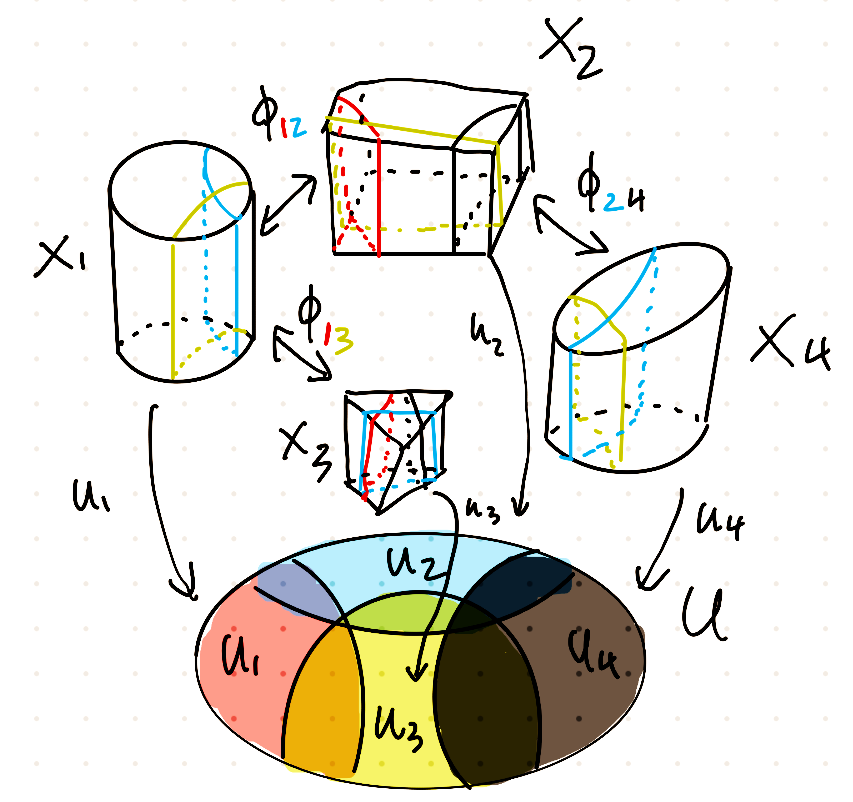
\includegraphics[width=11cm]{Images/Cocycle_condition.png}
\end{figure}
\end{remark}



\subsection{Descent data}

We are now ready to move onto stacks. The main idea is to generalize the type of \textit{local data} that we used to glue before.

For the rest of the chapter $\Cc$ is a site with a fixed Grothendieck topology and $\Fc$ is fibered category over $\Cc$.

\begin{definition}[]
Fix $U\in \Cc$ and a cover $\cpa{U_i\to U}\in \Cov(U)$. An \textbf{object with descent data} is a pair $(\cpa{\xi_i},\cpa{\phi_{ij}})$ where $\xi_i\in \Fc(U_i)$ for all $i$ and $\phi_{ij}:\pr_2^\ast\xi_j\to \pr_1^\ast\xi_i$ are isomorphisms which live in $\Fc(U_{ij})$ such that
\[\pr_{13}^\ast\phi_{ik}=\pr_{12}^\ast\phi_{ij}\circ \pr_{23}^\ast\phi_{jk}.\]
The $\phi_{ij}$ are called \textbf{transition isomorphisms}.
\end{definition}

If you are (very reasonably) getting confused with the pullbacks and indices, it may (or may not) be useful to admire \textit{the hypercube}
% https://q.uiver.app/#q=WzAsMTMsWzIsMSwiVV97amt9Il0sWzIsMywiVV97aWprfSJdLFsyLDQsIlVfaSJdLFsxLDQsIlVfe2lqfSJdLFszLDMsIlVfe2lrfSJdLFszLDEsIlVfayJdLFsxLDIsIlVfaiJdLFszLDUsIlxceGlfaSIsWzAsMTAwLDQ1LDFdXSxbMCw1LCJcXHByXzJeXFxhc3RcXHhpX2pcXHhyaWdodGFycm93e1xccGhpX3tpan19XFxwcl8xXlxcYXN0XFx4aV9pIixbMjM5LDEwMCw0MiwxXV0sWzAsMSwiXFx4aV9qIixbMCwxMDAsNDUsMV1dLFs0LDAsIlxceGlfayIsWzAsMTAwLDQ1LDFdXSxbMiwwLCJcXHByXzFee1xcYXN0fVxceGlfalxceGxlZnRhcnJvd3tcXHBoaV97amt9fVxccHJfMl5cXGFzdFxceGlfayIsWzIzOSwxMDAsNDIsMV1dLFs0LDMsIlxcYmVnaW57bWF0cml4fVxccHJfMl5cXGFzdFxceGlfa1xcXFxcXDtcXDtcXDtcXDtcXDtcXDtcXGRvd25hcnJvd3tcXHBoaV97aWt9fVxcXFxcXHByXzFeXFxhc3RcXHhpX2lcXGVuZHttYXRyaXh9IixbMjM5LDEwMCw0MiwxXV0sWzMsMiwiXFxwcl8xIl0sWzEsMywiXFxwcl97MTJ9IiwxXSxbMSw0LCJcXHByX3sxM30iLDFdLFs0LDIsIlxccHJfMSJdLFs0LDUsIlxccHJfMiIsMl0sWzEsMCwiXFxwcl97MjN9IiwxXSxbMCw1LCJcXHByXzIiXSxbMCw2LCJcXHByXzEiLDFdLFszLDYsIlxccHJfMiJdLFs3LDIsIiIsMSx7ImNvbG91ciI6WzAsMTAwLDQ1XSwic3R5bGUiOnsidGFpbCI6eyJuYW1lIjoibWFwcyB0byJ9fX1dLFs4LDksIiIsMCx7ImNvbG91ciI6WzIzOSwxMDAsNDJdfV0sWzksNiwiIiwxLHsiY29sb3VyIjpbMCwxMDAsNDVdLCJzdHlsZSI6eyJ0YWlsIjp7Im5hbWUiOiJtYXBzIHRvIn19fV0sWzgsMywiIiwxLHsib2Zmc2V0IjoyLCJjb2xvdXIiOlsyMzksMTAwLDQyXSwic3R5bGUiOnsidGFpbCI6eyJuYW1lIjoibWFwcyB0byJ9fX1dLFsxMCw1LCIiLDIseyJjb2xvdXIiOlswLDEwMCw0NV0sInN0eWxlIjp7InRhaWwiOnsibmFtZSI6Im1hcHMgdG8ifX19XSxbMTEsMCwiIiwyLHsib2Zmc2V0IjoyLCJjb2xvdXIiOlsyMzksMTAwLDQyXSwic3R5bGUiOnsidGFpbCI6eyJuYW1lIjoibWFwcyB0byJ9fX1dLFsxMSwxMCwiIiwwLHsiY29sb3VyIjpbMjM5LDEwMCw0Ml19XSxbMTIsNCwiIiwxLHsib2Zmc2V0IjoyLCJjb2xvdXIiOlsyMzksMTAwLDQyXSwic3R5bGUiOnsidGFpbCI6eyJuYW1lIjoibWFwcyB0byJ9fX1dLFsxMSw5LCIiLDAseyJjb2xvdXIiOlsyMzksMTAwLDQyXX1dLFs4LDcsIiIsMCx7ImNvbG91ciI6WzIzOSwxMDAsNDJdfV0sWzEyLDEwLCIiLDAseyJjb2xvdXIiOlsyMzksMTAwLDQyXX1dLFsxMiw3LCIiLDAseyJjb2xvdXIiOlsyMzksMTAwLDQyXX1dLFs4LDMsIiIsMSx7Im9mZnNldCI6LTIsImNvbG91ciI6WzIzOSwxMDAsNDJdLCJzdHlsZSI6eyJ0YWlsIjp7Im5hbWUiOiJtYXBzIHRvIn19fV0sWzEyLDQsIiIsMSx7Im9mZnNldCI6LTIsImNvbG91ciI6WzIzOSwxMDAsNDJdLCJzdHlsZSI6eyJ0YWlsIjp7Im5hbWUiOiJtYXBzIHRvIn19fV0sWzExLDAsIiIsMix7Im9mZnNldCI6LTIsImNvbG91ciI6WzIzOSwxMDAsNDJdLCJzdHlsZSI6eyJ0YWlsIjp7Im5hbWUiOiJtYXBzIHRvIn19fV1d
\[\begin{tikzcd}
	&& \textcolor{rgb,255:red,0;green,4;blue,214}{{\pr_1^{\ast}\xi_j\xleftarrow{\phi_{jk}}\pr_2^\ast\xi_k}} && \textcolor{rgb,255:red,230;green,0;blue,0}{{\xi_k}} \\
	\textcolor{rgb,255:red,230;green,0;blue,0}{{\xi_j}} && {U_{jk}} & {U_k} \\
	& {U_j} \\
	&& {U_{ijk}} & {U_{ik}} & \textcolor{rgb,255:red,0;green,4;blue,214}{\begin{array}{c} \begin{matrix}\pr_2^\ast\xi_k\\\;\;\;\;\;\;\downarrow{\phi_{ik}}\\\pr_1^\ast\xi_i\end{matrix} \end{array}} \\
	& {U_{ij}} & {U_i} \\
	\textcolor{rgb,255:red,0;green,4;blue,214}{{\pr_2^\ast\xi_j\xrightarrow{\phi_{ij}}\pr_1^\ast\xi_i}} &&& \textcolor{rgb,255:red,230;green,0;blue,0}{{\xi_i}}
	\arrow[color={rgb,255:red,0;green,4;blue,214}, from=1-3, to=1-5]
	\arrow[color={rgb,255:red,0;green,4;blue,214}, from=1-3, to=2-1]
	\arrow[shift right=2, color={rgb,255:red,0;green,4;blue,214}, maps to, from=1-3, to=2-3]
	\arrow[shift left=2, color={rgb,255:red,0;green,4;blue,214}, maps to, from=1-3, to=2-3]
	\arrow[color={rgb,255:red,230;green,0;blue,0}, maps to, from=1-5, to=2-4]
	\arrow[color={rgb,255:red,230;green,0;blue,0}, maps to, from=2-1, to=3-2]
	\arrow["{\pr_2}", from=2-3, to=2-4]
	\arrow["{\pr_1}"{description}, from=2-3, to=3-2]
	\arrow["{\pr_{23}}"{description}, from=4-3, to=2-3]
	\arrow["{\pr_{13}}"{description}, from=4-3, to=4-4]
	\arrow["{\pr_{12}}"{description}, from=4-3, to=5-2]
	\arrow["{\pr_2}"', from=4-4, to=2-4]
	\arrow["{\pr_1}", from=4-4, to=5-3]
	\arrow[color={rgb,255:red,0;green,4;blue,214}, from=4-5, to=1-5]
	\arrow[shift right=2, color={rgb,255:red,0;green,4;blue,214}, maps to, from=4-5, to=4-4]
	\arrow[shift left=2, color={rgb,255:red,0;green,4;blue,214}, maps to, from=4-5, to=4-4]
	\arrow[color={rgb,255:red,0;green,4;blue,214}, from=4-5, to=6-4]
	\arrow["{\pr_2}", from=5-2, to=3-2]
	\arrow["{\pr_1}", from=5-2, to=5-3]
	\arrow[color={rgb,255:red,0;green,4;blue,214}, from=6-1, to=2-1]
	\arrow[shift right=2, color={rgb,255:red,0;green,4;blue,214}, maps to, from=6-1, to=5-2]
	\arrow[shift left=2, color={rgb,255:red,0;green,4;blue,214}, maps to, from=6-1, to=5-2]
	\arrow[color={rgb,255:red,0;green,4;blue,214}, from=6-1, to=6-4]
	\arrow[color={rgb,255:red,230;green,0;blue,0}, maps to, from=6-4, to=5-3]
\end{tikzcd}\]



\begin{notation}[]
Let $\Cc$ be a site, $\Fc$ fibered over $\Cc$, $U\in \Cc$ and $\cpa{U_i\to U}\in \Cov(U)$. Objects with descent data over $\cpa{U_i\to U}$ form a category\footnote{the morphisms are collections of maps and commutative diagrams which are compatible with the indices.}, which we denote using 
\[\Fc(\cpa{U_i\to U}).\]
\end{notation}


\begin{remark}
Fix $U\in \Cc$, $\cpa{u_i:U_i\to U}\in \Cov(U)$ and $\xi\in \Fc(U)$. From $\xi$ we can obtain an object with descent data by restriction. To be more precise, we can define
\[\xi_i=u_i^\ast\xi,\qquad \phi_{ij}:\pr_2^\ast u_j^\ast\xi\to \pr_1^\ast u_i^\ast \xi\]
where $\phi_{ij}$ is the canonical isomorphism induced by the fact that both objects amount to the pullback of $\xi$ along $U_{ij}\to U$. The resulting object with descent data is $(\cpa{\xi_i},\cpa{\phi_{ij}})$.
\end{remark}

\begin{center}
\textit{What we have described is actually a functor from $\Fc(U)$ to $\Fc(\cpa{U_i\to U})$.}
\end{center}

\begin{definition}[]
An object with descent data is called \textbf{effective} if it is in the essential image of the functor above.
\end{definition}

\noindent We are now finally ready to define prestacks and stacks:
\begin{definition}[]
Let $\Fc$ be a fibered category over $\Cc$ site. $\Fc$ is a
\begin{itemize}
	\item \textbf{prestack} if for all $U\in \Cc$ and all $\cpa{U_i\to U}\in \Cov(U)$, the functor
	\[\Fc(U)\to \Fc(\cpa{U_i\to U})\]
	is \textit{fully faithful}.
	\item \textbf{stack} if for all $U\in \Cc$ and all $\cpa{U_i\to U}\in \Cov(U)$, the functor
	\[\Fc(U)\to \Fc(\cpa{U_i\to U})\]
	is an \textit{equivalence}.
\end{itemize}
\end{definition}

\begin{remark}
The two conditions can be intuitively understood as:
\begin{itemize}
\item A prestack is a fibered category where if two objects are the same locally (taking into account gluing) then they are isomorphic.
\item A stack is a prestack where all descent data glues to an object.
\end{itemize}
\end{remark}

Another way in which we can intepret the prestack condition is given in the following

\begin{proposition}
Let $\Fc$ be fibered over $\Cc$ site. $\Fc$ is a prestack if and only if for all $U\in \Cc$ and all $\xi,\eta\in \Fc(U)$, the functor
\[\ul{\Hom}_U(\xi,\eta):\funcDef{(\Cc/U)\op}{\Set}{f:Z\to U}{\Hom_Z(f^\ast\xi,f^\ast \eta)}\]
is a sheaf on $\Cc/U$.
\end{proposition}
\begin{proof}[Sketch]
Fix $U\in \Cc$ and $\cpa{U_i\to U}\in \Cov(U)$. The functor $\Fc(U)\to \Fc(\cpa{U_i\to U})$ being fully faithful means that for all $\xi,\eta\in \Fc(U)$ we have
\[\Hom_U(\xi,\eta)\cong \Hom_{\cpa{U_i\to U}}((\cpa{\xi_i},\cpa{\al_{ij}}),(\cpa{\eta_i},\cpa{\beta_{ij}}))\]
where $(\cpa{\xi_i},\cpa{\al_{ij}})$ is the image of $\xi$ and similarly for the other object and $\eta$.

Concretely, this means that maps $\xi\to \eta$ can be defined uniquely on an open cover, which is exactly what it means for $\ul{\Hom}_U(\xi,\eta)$ to be a sheaf.
\end{proof}

\begin{corollary}
$\Arr(\Top)$ is a stack.
\end{corollary}

We close the chapter by noting that when $\Fc/\Cc$ is fibered in sets, we find the notions of separated presheaf and sheaf over $\Cc$ respectively, meaning that we have, in some very precise sense, defined \textit{sheaves in categories}. This concept will be trated in more detail in the next chapter.
\begin{proposition}
Let $\Cc$ be a site and consider a functor $F:\Cc\op\to \Set$. Identify $F$ with the fibered category it defines. Then
\begin{itemize}
	\item $F$ is a prestack if and only if it is a separated presheaf,
	\item $F$ is a stack if and only if $F$ is a sheaf.
\end{itemize}
\end{proposition}

\begin{example}
The fibered category associated to an object $X\in \Cc$ is a stack because it corresponds to the functor $h_X=\Hom_\Cc(\cdot, X)$.
\end{example}


